\documentclass{standalone}
\usepackage{tikz}
\usepackage{pgfplots,pgfplotstable,}
\usetikzlibrary{pgfplots.colorbrewer}
\usepgfplotslibrary{patchplots}
\usetikzlibrary{calc,arrows,arrows.meta,shapes,shadows,shapes.arrows,spy,angles,animations,backgrounds,decorations,patterns,babel,bending,}
\usepackage{amsmath,amsfonts,amssymb,xfrac,cancel}
\usepackage{xcolor}
\usepackage{xkeyval}
\usepackage{tikz-3dplot}
\usepackage{rotating}
\usetikzlibrary{fadings, decorations.markings}

%rotate=5,transform shape
%rotate=5,rotate around y=15,transform shape
\begin{document}
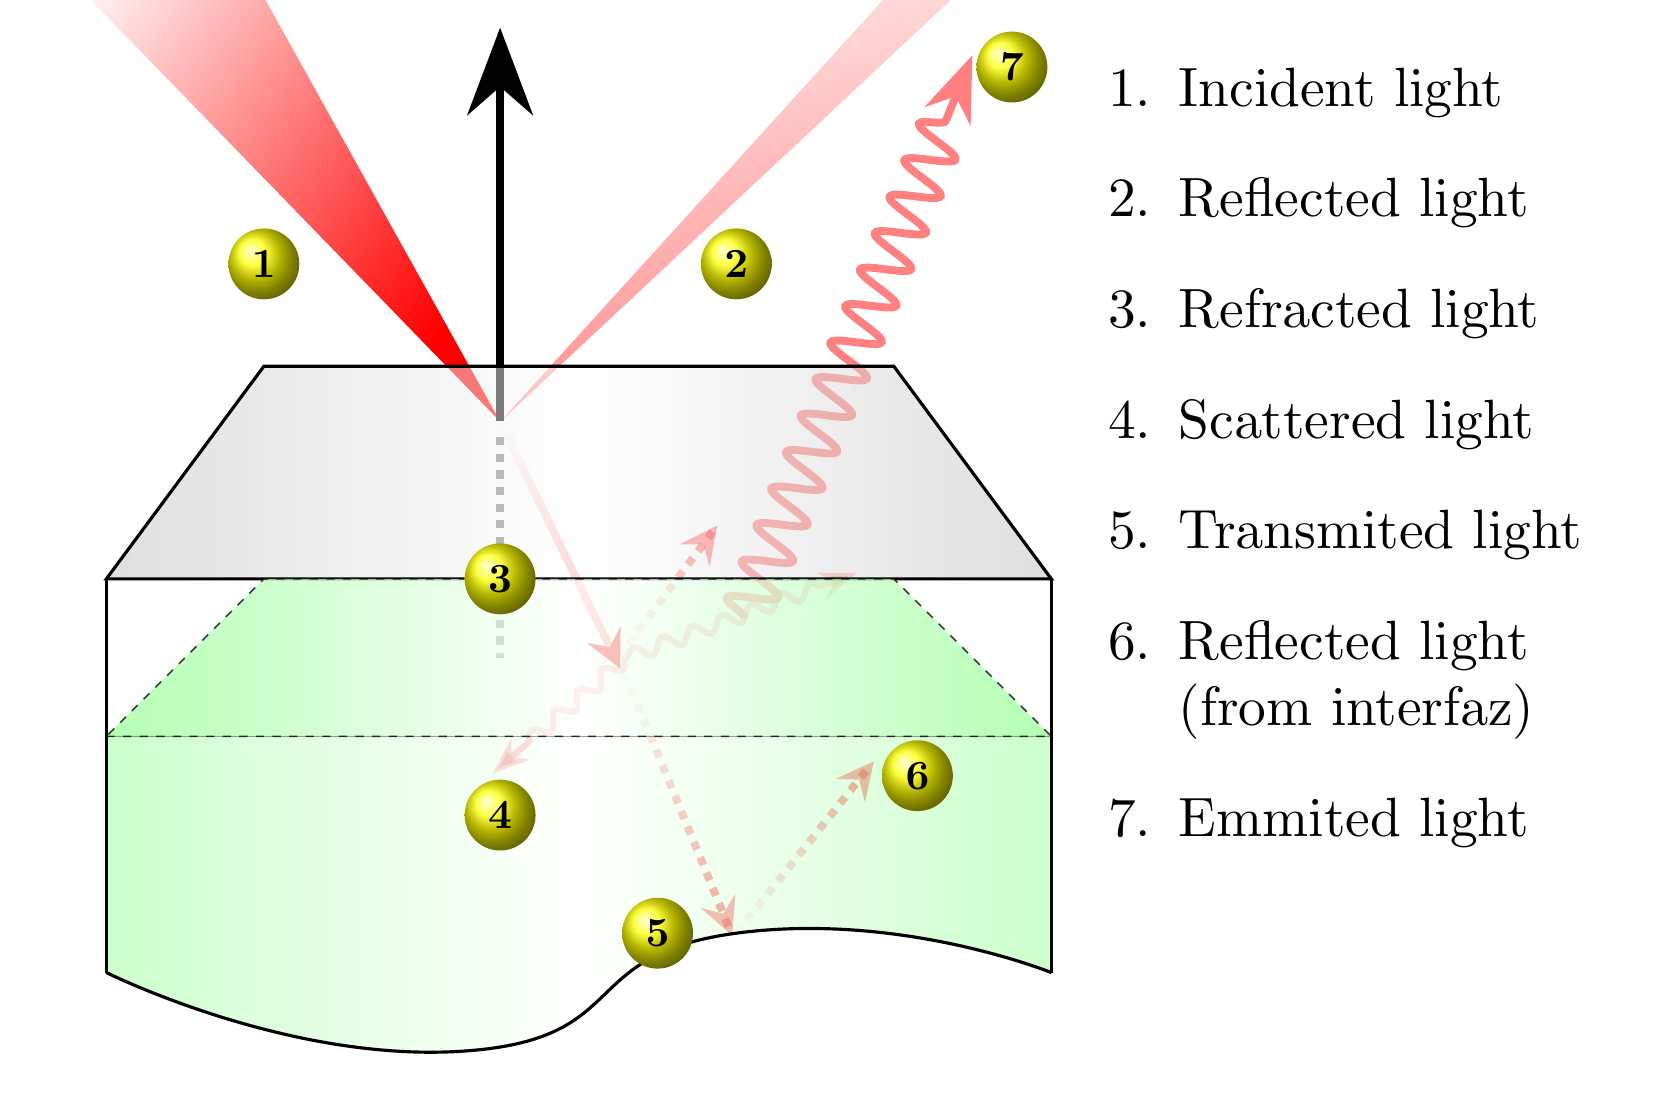
\begin{tikzpicture}[decoration={snake,amplitude=.9mm,
		segment length=4mm,post length=4mm},rotate=0,rotate around y=45,transform shape]


\useasboundingbox (-70mm,7mm) rectangle (135mm,140mm);



\fill[color=red, path fading=north,fading transform={rotate=45}] (-50mm,140mm) ++(135:2) ++(225:0.3) -- ++(45:2) -- (-10mm,90mm) -- cycle;%incident

\fill[color=red, path fading=north,fading transform={rotate=15},opacity=0.5]
(40mm,130mm) ++(60:3) ++(150:0.1) -- ++(-30:1) -- (-10mm,90mm) -- cycle;%reflected


\draw[red,
decoration={markings,mark=at position 1 with {\arrow[scale=1.5,red]{stealth}}},
preaction={decorate},
shorten >=5mm, path fading=north,
line width=1mm,
opacity=0.5
] (-10mm,90mm) -- (7mm,55mm);

%
\draw[red,
decoration={markings,mark=at position 1 with {\arrow[scale=1.5,red,opacity=0.5]{stealth}}},
preaction={decorate},
shorten >=5mm, 
path fading=south,
line width=1mm,
opacity=0.75,dashed
]  (5mm,60mm)--(20mm,80mm);


\draw[decorate,red,-{Stealth},line width=0.8mm,opacity=0.25] (6mm,60mm) -- ++(5:3);%  dispersion

\draw[decorate,red,-{Stealth},line width=0.8mm,opacity=0.25] (6mm,60mm) -- ++(210:2);% dispersion

\draw[red,
decoration={markings,mark=at position 1 with {\arrow[scale=1.5,red,opacity=0.5]{stealth}}},
preaction={decorate},
shorten >=5mm, path fading=north,
line width=1mm,
opacity=0.75,dashed
]  (5mm,60mm)--(21mm,21mm);



\draw[red,
decoration={markings,mark=at position 1 with {\arrow[scale=1.5,red,opacity=0.5]{stealth}}},
preaction={decorate},
shorten >=5mm, path fading=south,
line width=1mm,
opacity=0.75,
transform shape,dashed
]  (20mm,25mm)--(40mm,50mm);


\draw[decorate,red!50,-{Stealth[scale=1.5]},decoration={snake,amplitude=3mm,
	segment length=5mm,post length=7mm},line width=1mm,opacity=1] (21mm,65mm) -- ++(65:7);% emithed



\draw[-{Stealth[scale=2]},line width=1mm] (-10mm,90mm)--(-10mm,140mm);

\draw[line width=1mm,dashed,opacity=0.5] (-10mm,88mm)--(-10mm,60mm);


\draw[left color=black!25, right color=black!25, middle color=white,fill opacity=0.5,line width=0.4mm] (-60mm,70mm)--(60mm,70mm)--(40mm,97mm)--(-40mm,97mm)--cycle;
%\draw (-50mm,70mm)--(-45mm,20mm);
%\draw (45mm,70mm)--(45mm,30mm);


\draw [black,left color=green!40, right color=green!40, middle color=white,opacity=0.5] plot [smooth,tension=1] coordinates { (-60mm,20mm) (-15mm,10mm) (20mm,25mm) (60mm,20mm)}--(60mm,50mm)--(-60mm,50mm)--cycle;




\draw[left color=green!40, right color=green!40, middle color=white,opacity=0.75,line width=0.2mm,dashed] (-60mm,50mm)--(60mm,50mm)--(40mm,70mm)--(-40mm,70mm)--(-60mm,50mm);



%\draw[dashed] (-60mm,50mm)--(60mm,50mm)--(40mm,70mm)--(-40mm,70mm)--(-60mm,50mm);

\draw [black,line width=0.4mm,opacity=1] plot [smooth,tension=1] coordinates { (-60mm,20mm) (-15mm,10mm) (20mm,25mm) (60mm,20mm)};

\draw[line width=0.4mm] (-60mm,20mm)--(-60mm,70mm);
\draw[line width=0.4mm] (60mm,20mm)--(60mm,70mm);


\shade[ball color=yellow] (-40mm,110mm) circle (4.5mm) node[font=\bf,scale=1.5] {1};
\shade[ball color=yellow] (20mm,110mm) circle (4.5mm) node[font=\bf,scale=1.5] {2};
\shade[ball color=yellow] (-10mm,70mm) circle (4.5mm) node[font=\bf,scale=1.5] {3};
\shade[ball color=yellow] (-10mm,40mm) circle (4.5mm) node[font=\bf,scale=1.5] {4};
\shade[ball color=yellow] (10mm,25mm) circle (4.5mm) node[font=\bf,scale=1.5] {5};
\shade[ball color=yellow] (43mm,45mm) circle (4.5mm) node[font=\bf,scale=1.5] {6};
\shade[ball color=yellow] (55mm,135mm) circle (4.5mm) node[font=\bf,scale=1.5] {7};


\node[anchor=center,
	text width=0.3\linewidth,
	scale=2] at (95mm,90mm){
	\begin{enumerate}
	\item Incident light
	\item Reflected light 
	\item Refracted light
	\item Scattered light
	\item Transmited light
	\item Reflected light (from interfaz)
	\item Emmited light
	\end{enumerate}};


\end{tikzpicture}
\end{document}